\documentclass[11pt]{article}
%%%%%%%%%%%%%%%%%%%%%%%%%%%%%%%%%%%%%%%%%

\usepackage{amscd}
\usepackage{amsmath}
\usepackage{amssymb}
\usepackage{amsthm}


\usepackage{epsfig}
\usepackage{verbatim}
\usepackage{graphicx}
\usepackage{amsthm}
\usepackage{multirow}
\usepackage{hyperref}
\pagestyle{empty}
\usepackage{color}
\usepackage[left=3cm,top=2.5cm,right=3cm,bottom=3cm]{geometry} % Document margins
%\usepackage[all,dvips]{xy}


\begin{comment}  

This LaTeX document is a template to be used by Bates mathematics rising seniors to create a thesis proposal. 

As a guide, the document is already filled out to represent a fictitious proposal, and all you need to do is modify the entries below to represent your own proposal.

A PDF version of the fictitious proposal is available on the department's FAQ and Policies pages, at
http://abacus.bates.edu/acad/depts/math/faq.html
and
http://abacus.bates.edu/acad/depts/math/policies.html
respectively.

Once you have finished your proposal, export it to a PDF file. Give the file a USEFUL name, for example, RiemannThesisProposal.PDF. Email the PDF file to Clementine Brasier, the 
Academic Administrative Assistant for Hathorn Hall, at cbrasier\@bates.edu

This LaTex document was created Feb/Mar 2010 by Adriana Salerno and updated Feb 2012 by Meredith Greer

\end{comment}


%%%%%%%%%%%%%%%%%%%%%%%%%%%%%%%%%%%%%%%%%

\begin{document}
	\begin{titlepage}
		\centering
		
\includegraphics[width=0.15\textwidth]{NU_logo.png}\par\vspace{1cm}
		{\scshape\LARGE Northeastern University \par}
		\vspace{1cm}
		{\scshape\Large Data Mining Project Report (Draft)\par}
		\vspace{1.5cm}
		{\huge\bfseries Recommendation Systems for Yelp Dataset\par}
		\vspace{2cm}
		{\Large\itshape Aditya Priyadarshi, Abhay Kasturia, Xingxing Liu, Varun Nandu and Gautam Vashisht \par}
		%{\Large\itshape (priyadarshi.a@husky.neu.edu) \par}
		\vfill
		Supervised by\par
		Dr. Nate \textsc{Derbinsky}
		
		\vfill
		
		% Bottom of the page
		{\large \today\par}
	\end{titlepage}
	
	\section{Introduction and Related Work}
		A recommender system or a recommendation system is a subclass of information filtering systems that seeks to predict the rating or preference that a user would give to an item \cite{rsw}. Recommendations systems have become very relevant today given the presence of e-commerce website like Amazon and Netflix as well as other platforms like Facebook and Youtube. These are utilized in a variety of areas such as movies, music, videos, news, books, research articles, search queries and products in case of Amazon. Two most common methods to build a recommendation system are collaborative filtering and content-based filtering. Collaborative filtering methods use user's past behaviors and behaviors of similar users to find items which a user might like. Content-based methods use the features of the items liked by the user to suggest similar items. There are also hybrid recommendation system which combine both of these techniques.
	
	\bigskip
	
	
	\section{Dataset and Analysis} 
		\subsection{Dataset}
		 The original dataset described in the Yelp Dataset Challenge 10 \cite{yelp} has 4.7M reviews and 1M tips by 1.1M users for 156K businesses spread across 12 cities. The 	data is given in json format which include business.json, review.json, user.json, checkin.json and tip.json.Each business has name, address, star rating and textual reviews. Each individual review data consists of anonymized IDs for the business, user and review, star rating, review type, review text and votes on how useful, funny or cool the review is.
		\begin{figure}[h]
				\centering
				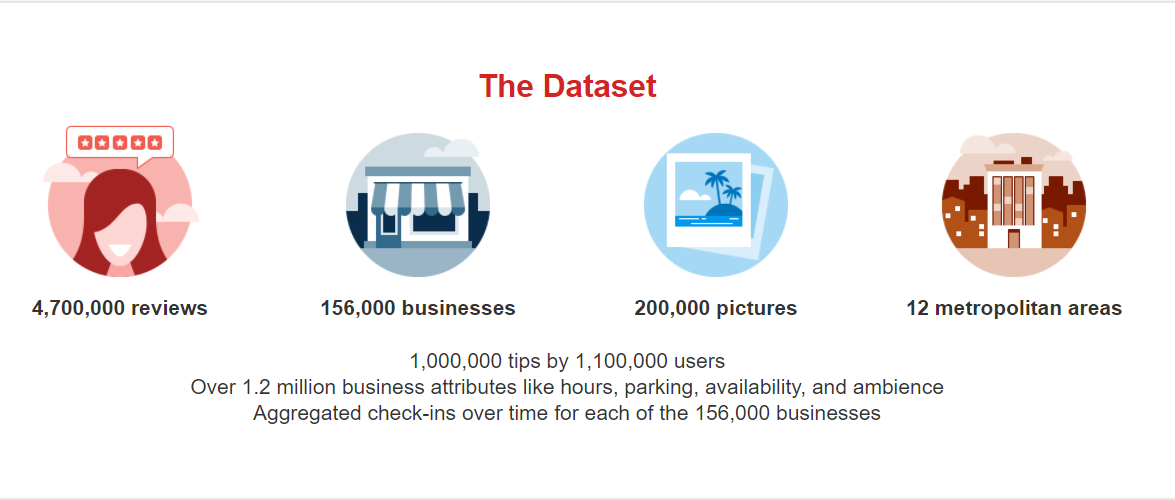
\includegraphics[scale=0.5]{data_details.png}
				\caption{Dataset Details}
		\end{figure}
		\subsection{Analysis}
		We did an initial analysis of the dataset. Below sections present our analysis.
			\subsubsection{User data}
			There are 1183362 total users whose reviews are present in the dataset. We plotted a histogram to understand the distribution of user reviews. Looking at the histogram, we can observe that most of the user have very few reviews and some top users have significant number of reviews. Majority of user have 25 or less reviews which is also shown by a mean of 23..72 and standard deviation of 80.5. The maximum number of reviews given by any user is 11656.
		
			\begin{figure}[h]
					\centering
					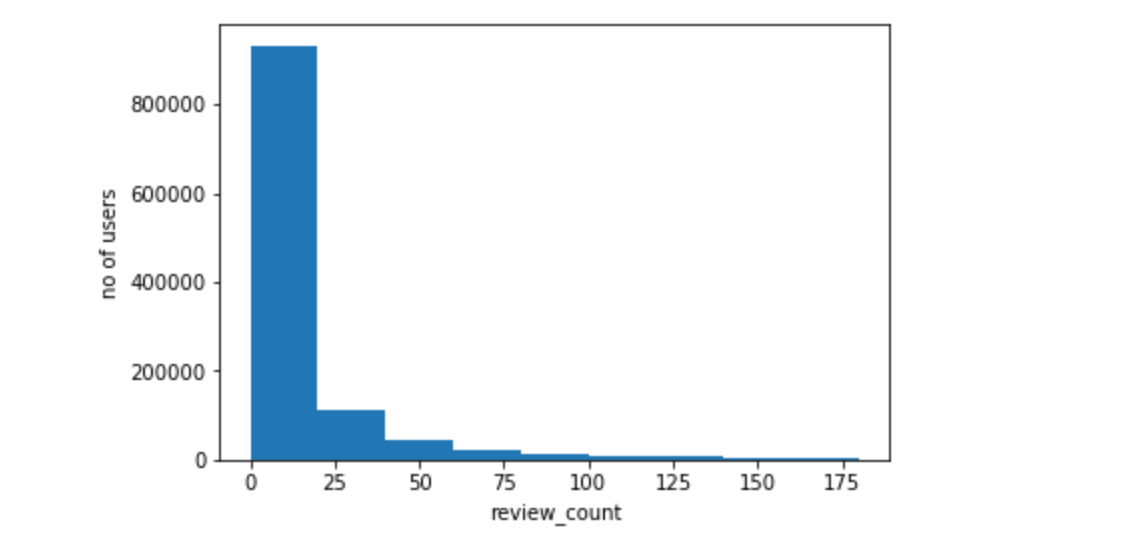
\includegraphics[scale=0.5]{h_user_review.png}
					\caption{Review count per user}
			\end{figure}
		  In addition to number of reviews, we also looked at distribution of star ratings given by a user. Looking at the histogram, we can observe that more users give higher rating which is shown by a median of 3.89 star rating. Mean and standard deviation for the same are 3.71 and 1.10 respectively. In order to group the reviews as positive, average and negative reviews, we have used the following method. We assume that if the rating lies in the range of (mean – standard deviation, mean) which is 2.6 to 3.7, we will categorize it as average. Reviews lower than 2.6 will be considered as a negative review and anything greater than 3.7 will be considered as positive reviews with two extremes being 0 and 1. 
		 
		  \begin{figure}[h]
		  	\centering
		  	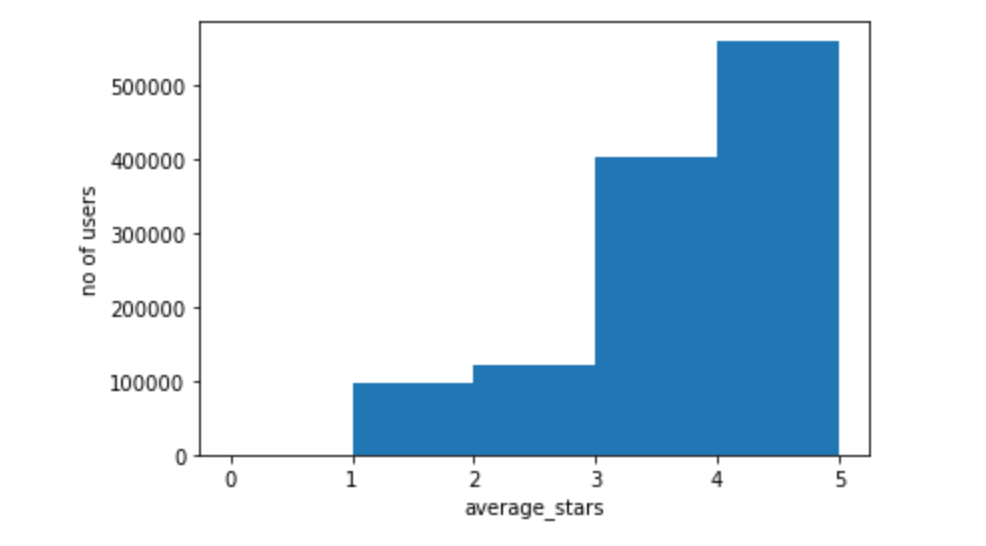
\includegraphics[scale=0.7] {h_user_rating.png}
		  	\caption{Rating per user}
		  \end{figure}
	     We also did some analysis to see the user growth on yelp. User growth has started declining after an increase in users joining from 2005 to 2014 .
	     
	      \begin{figure}[h]
	     	\centering
	     	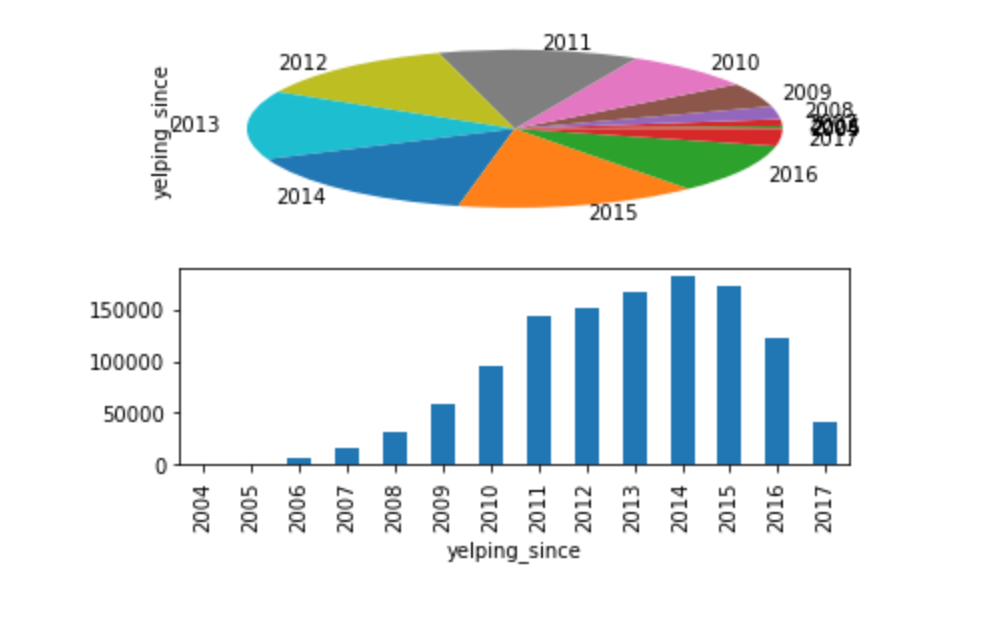
\includegraphics[scale=0.5] {user_growth.png}
	     	\caption{User Growth}
	     \end{figure}
     
     	\subsubsection{Business Data}
     	There are total 156639 business in the dataset. We grouped business according to city and business category to determine popular cities and categories. Below pie-charts give idea about popular cities and categories.
     	
     	\begin{figure}[h]
     		\centering
     		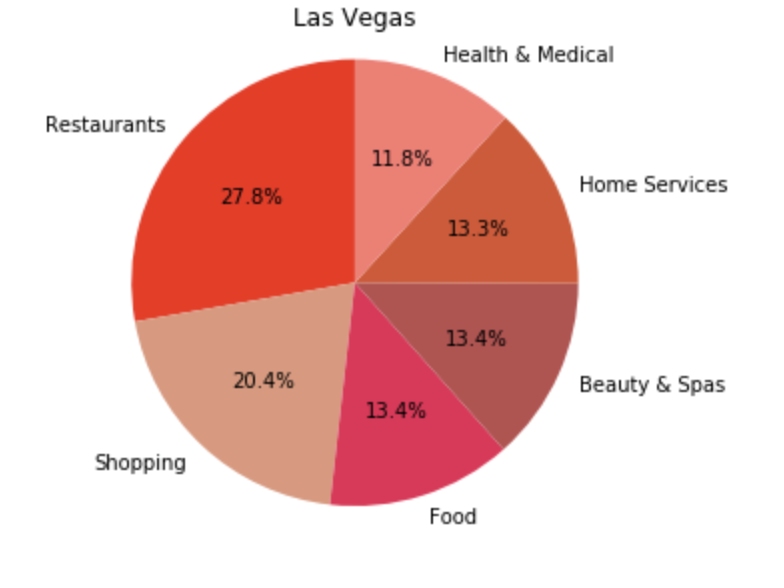
\includegraphics[scale=0.7] {top_cities.png}
     		\caption{Top cities}
     	\end{figure}
	     \begin{figure}[h]
	     	\centering
	     	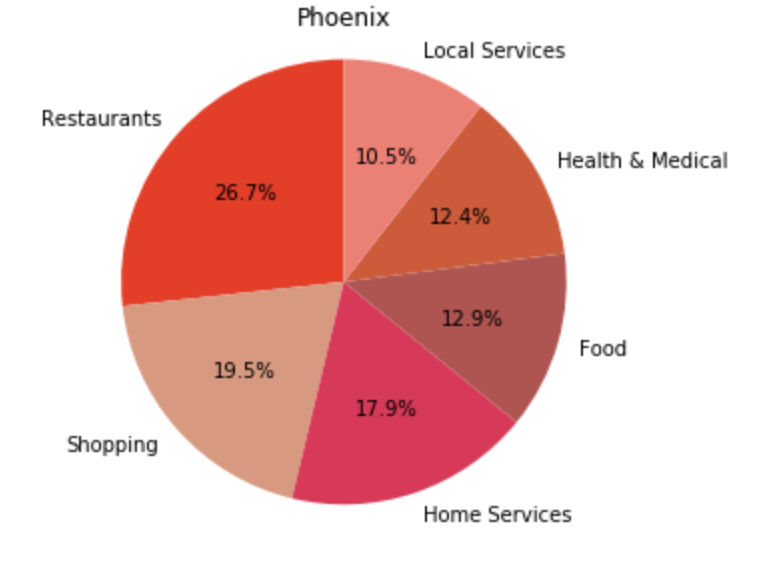
\includegraphics[scale=0.7] {top_categroies.png}
	     	\caption{Top Business Categories}
	     \end{figure}
     We did more analysis into sub-categories of our most popular category i.e. restaurants to map its distribution.
      \begin{figure}[h]
     	\centering
     	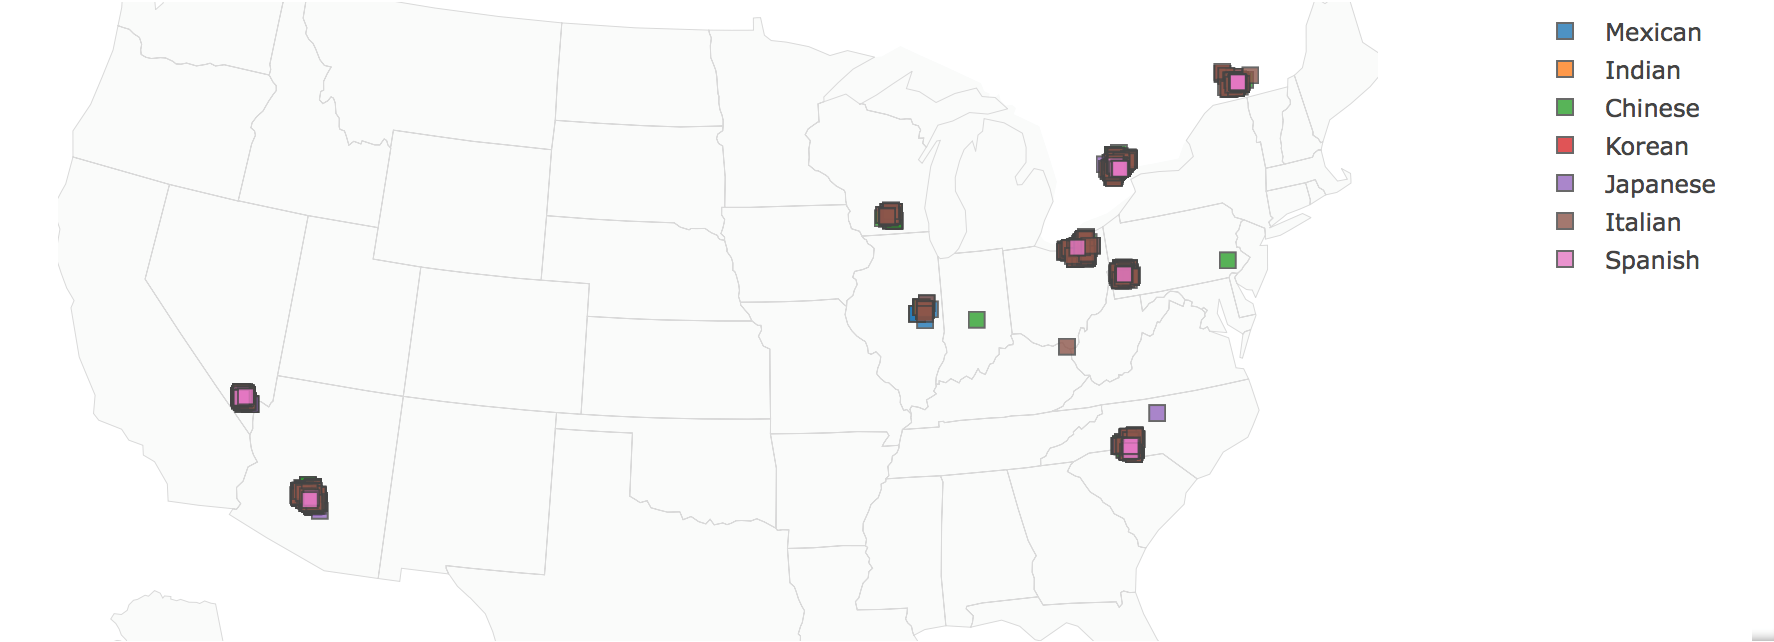
\includegraphics[scale=0.5] {category_map.png}
     	\caption{Restaurant Sub-categories}
     \end{figure}
      

 	\subsubsection{Checkin Data}
 	Finally, we did analysis on use checkin data to find out popular timing in the top cities shown in our earlier analysis.
 
      \begin{figure}[h]
 		\centering
 		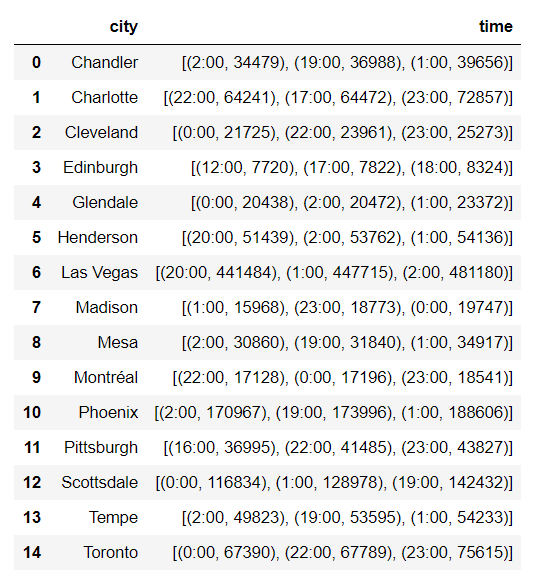
\includegraphics[scale=0.5] {checkin_times.png}
 		\caption{Checkin Times}
 	\end{figure}
 	
	\section{Methods}
		
		\subsection{Clustering Based Approach}
		Clustering is based on the reviews of users. From the reviews we can build vector for each user and business with preference on different categories of businesses. By computing the distance of these two vectors, we can recommend businesses to user with the most similar preference vector value.
		There are basically four steps:- 
		\begin{enumerate}
			\item  compose the preference vector of both users and businesses.
			\item  clustering on user to generate a more general user preference vector
			\item  calculating similarity of user preference and business preference
			\item  Generating recommendations
		\end{enumerate}
		
		\subsubsection{Vector Calculating}
		Preference Vector is built on a common top 20 categories of a certain type of business such as 'Restaurant'. That's saying 20 kinds of restaurant like 'Spanish', 'Chinese', 'Mexican', 'Indian' and so on.
		 \begin{figure}[h]
			\centering
			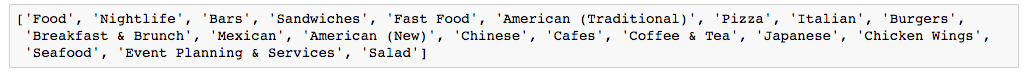
\includegraphics[scale=0.5] {vector1.png}
			\caption{Top 20 Categories}
		\end{figure}
	
		Based on users' each review, we can get the preference rating from 1 to 5 for a particular business, from which we can generate a rating value for each of the category in that particular business. For those categories user does not have review on, we assign a value of 1. Thus we get a vector of rating value on all top 20 categories for each user. The same procedure goes to business.
		Vector comes with format '[1,2,3, ...]', with respect to a list of categories '[Indian, Chinese, Mexican, Spanish, ...]'.
		 \begin{figure}[h]
			\centering
			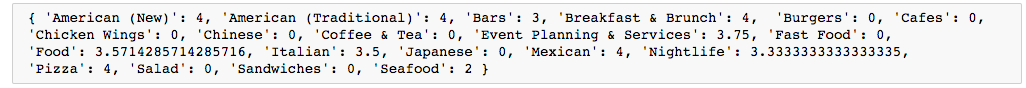
\includegraphics[scale=0.5] {vector2.png}
			\caption{Top 20 Categories}
		\end{figure}
		
		\subsubsection{Clustering on Users}
		Given the vector of each user, we can calculate the Euclidean distance of each pair of users. Then perform average agglomerative clustering on the users' distance matrix. Dendogram after performing clustering on 8000 users is as shown in figure. Based on the above dendogram we can decide on a cut-off point to get number of clusters. For the above dendogram we selected 10 clusters. 
		 \begin{figure}[h]
			\centering
			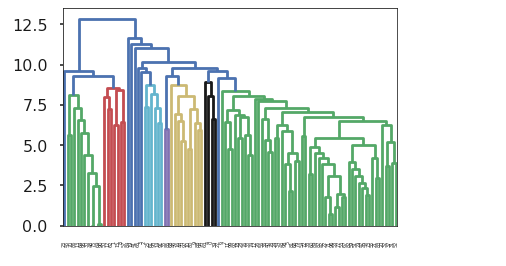
\includegraphics[scale=0.5] {dendogram.png}
			\caption{Dendogram after Clustering}
		\end{figure}
		
		\subsection{Collaborative Filtering}
		Collaborative Filtering is the method to implement recommendation system. It is the way to recommend item to user 'u1' by collaborating the choice of item of other users similar to user 'u1'. We create a n X m matrix, where n is the number of users and m is the number of business, with each cell representing the rating given by a user to that particular business. Each row in matrix represent the vector of star rating given by user for all the businesses. \\
	 
	 		\begin{figure}[h]
					\centering
					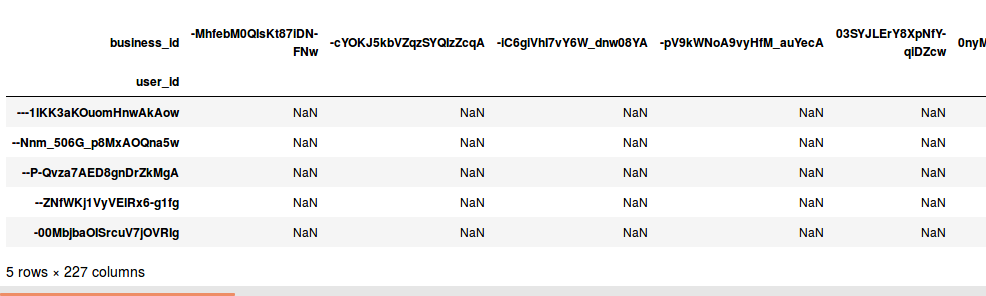
\includegraphics[scale=0.5]{uservsitem.png}
					\caption{UserVsBusiness - Stars Rating Value}
			\end{figure}
	 
		While doing this, we face two issues 
		1. As expected, there are a lot of missing values in matrix(for items which user has not given rating). We treat missing values as the average computed after following the second step - which will always be zero.
		2. There is an issue of handling the rating given by soft users and hard users i.e some users may rate the business they like with a 3 star ratings and there are some users who may rate the business they don't like with a 3 star ratings. To normalize these ratings for each user we use the centered cosine similarity. We normalize the ratings by subtracting the row mean for each user.\cite{vid1}\\
		
		To recommend new businesses to a target user 'target', we find the cosine similarity between all other users and 'target'. Top 'k' businesses rated with positive average star rating, by users of having cosine similarity greater than 1, will be recommended to user 'target'.\cite{vid2}
	
		\subsection{Collaborative Deep Learing} 
		We are using Collaborative Deep Learning \cite{cdl} (CDL) approach suggested by Hao Wang and team. We looked at various deep learning approaches towards building recommendation systems and we choose this work as it was generally applicable compared to other techniques which either target music or videos recommendations. CDL is a hierarchical Bayesian model. Stacked Denoising autoencoders \cite{sdae} are used for feature learning and cleaning the noise from the input. In below sections, I will be brief about the input parameters and neural network architecture.
		
		\subsubsection{Notation and Problem Formulation}
		As explained in \cite{cdl}, collection of J items (business) is represented by J-by-S matrix $X_c$, where row j is the bag-of-words vector $X_{c,j*}$ for item j based on a vocabulary size S. Assuming I users, an I-by-J rating matrix R. Given part of the ratings in R and the content information Xc, the problem is to predict the other ratings in R. Here, $X_c$ is the clean matrix after using SDAE and $X_o$ is the noise-corrupted matrix.
		  
		\subsubsection{Stacked Denoising Autoencoders}
		SDAE \cite{sdae} is a feedforward neural network for learning representations (encoding) of the input data by learning to predict the clean input itself in the output as shown in figure
		\begin{figure}[h]
			\centering
			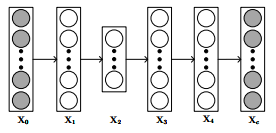
\includegraphics[scale=0.7]{sdae.png}
			\caption{Stacked Denoising Autoencoders}
		\end{figure}
		
		\subsubsection{Collaborative Deep Learing Model}
		Below figures show the model in detail, where W is weight matrix. The part inside the dashed rectangle represents an SDAE. An example SDAE with L=2 is shown. Here, $\lambda_w$, $\lambda_n$, $\lambda_u$, $\lambda_s$ and $\lambda_v$ are hyper-parameters. The middle layer $X_{L/2}$ serves as a bridge between the ratings and content information. 
		
		\begin{figure}[h]
			\centering
			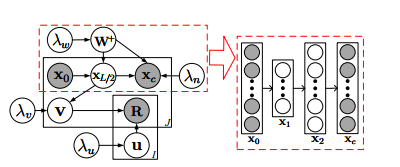
\includegraphics[scale=0.7]{cdl.png}
			\caption{Graphical model of CDL}
		\end{figure}
		\begin{figure}[h]
			\centering
			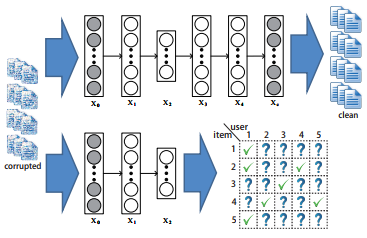
\includegraphics[scale=0.7]{cdl1.png}
			\caption{NN representation for degenerated CDL}
		\end{figure}
	\section{Experiments and Results}
	\subsection{Clustering Based Approach}
	\subsubsection{Calculating Similarity and Generating Recommendations}
	Based on users clustering dendogram shown in figure, we generate an average vector representing user preference vector. Then we Do an inner product of user vector and business vector. Smaller the value, more similar the user and the business. From the results, we choose top 10 or 20 business with the minimum value as the recommendations. Below is a sample for user with user is: 'McLqvYLBQoCFQikU9dC4cQ' searching for “Restaurants”.

	\begin{figure}[h]
		\centering
		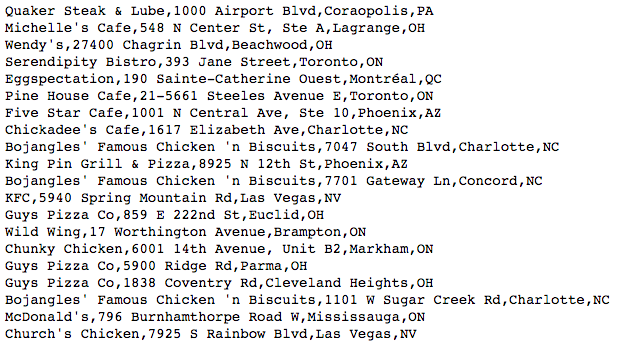
\includegraphics[scale=0.7]{results_cl.png}
		\caption{Results for User with id 'McLqvYLBQoCFQikU9dC4cQ'}
	\end{figure}
	
	\subsubsection{Evaluation of the clustering}
	We used cophenetic correlation to evaluate the quality of the clustering. 
	\begin{figure}[h]
		\centering
		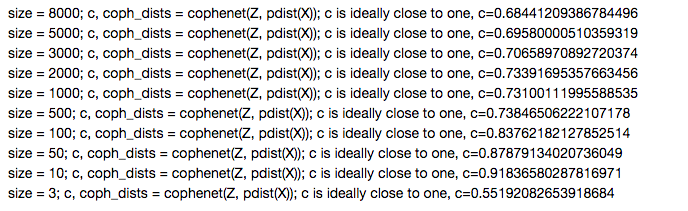
\includegraphics[scale=0.7]{eval_cl.png}
		\caption{Cophenetic Correlation Distance for Different User Groupings}
	\end{figure}
	\subsection{User-User Collaborative Filtering}

	For the initial setup, we have worked on 100,000 rows of reviews.json file. We have created a matrix of 78276 users and 4224 businesses.We randomly choose one user to find the set of similar users of count 200. Based on positive average star ratings given by 200 users, 531 set of businesses are recommended to users.
	
	
	
	\section{Future work}
	\begin{enumerate}
		\item Modify original collaborative deep learning implementation\cite{cdli} of paper \cite{cdl} to analyze our dataset.
		\item All the algorithms are run on a small subset of data. Look into distributive processing framework(Spark), to perform the same on all the data or leverage the Google Cloud Platform.
		\item Finalize evaluation criteria. The general approach that we plan to take would be:
		\begin{enumerate}
			\item Divide training and test data based on the timeline of reviews - to get past activity and future activity.
			\item Define users in future activity as target users. Use the past activity of the target users to make recommendations.
			\item Evaluate the recommendation as correct, if the recommendation shows up in the users future activity.
			\item Get the total accuracy based on the same and evaluate our model!
		\end{enumerate}
		\item Handle the problem of cold  start - where a new business or a user is added. The general approach here would be to recommend the most popular business to the new user. Have to search for a way to tackle new businesses.
		
	\end{enumerate}
	
	\begin{thebibliography}{99}
		% NOTE: change the "9" above to "99" if you have MORE THAN 10 references.
		
	\bibitem{yelp} Yelp Dataset Challenge \url{https://www.yelp.com/dataset_challenge}
	\bibitem{rsw} Recommendation System Wiki \url{https://en.wikipedia.org/wiki/Recommender_system}
	\bibitem{cfilter}Collaborative filtering \url{https://en.wikipedia.org/wiki/Collaborative_filtering}
		\bibitem{cfiltervid}Collaborative filtering Techniques \url{https://www.youtube.com/watch?v=h9gpufJFF-0}
		\bibitem{mov}Movie Recommenation System \url{https://beckernick.github.io/matrix-factorization-recommender/}
	\bibitem{ydeep} Paul Covington, Jay Adams, Emre Sargin \textit{Deep Neural Networks for YouTube Recommendations}, ACM 2016.
	\bibitem{cdl} Hao Wang, Naiyan Wang, Dit-Yan Yeung\textit{Collaborative Deep Learning for Recommender Systems}, ACM 2015
	\bibitem{vid1} Lecture on CF - Stanford \url{https://www.youtube.com/watch?v=h9gpufJFF-0&t=854s}
	\bibitem{vid2} Recommendation System Netflix \url{https://www.youtube.com/watch?v=bLhq63ygoU8&t=5598s}
	\bibitem{sdae} P. Vincent, H. Larochelle, I. Lajoie, Y. Bengio, and
	P.-A. Manzagol. \textit{Stacked denoising autoencoders:
		Learning useful representations in a deep network with
		a local denoising criterion.} JMLR, 11:3371–3408, 2010
	\bibitem{cdli} CDL Implementation \url{https://github.com/hexiangnan/neural_collaborative_filtering}
	\end{thebibliography}
	%%%%%%%%%%%%%%%%%%%%%%%%%%%%%%%%%%%%%%%%%
	
	
	
	
	
	
\end{document} 